\documentclass[sigconf]{acmart}

\usepackage{hyperref}

%\usepackage{endfloat}
%\renewcommand{\efloatseparator}{\mbox{}} % no new page between figures

\usepackage{booktabs} % For formal tables

\settopmatter{printacmref=false} % Removes citation information below abstract
\renewcommand\footnotetextcopyrightpermission[1]{} % removes footnote with conference information in first column
\pagestyle{plain} % removes running headers


%\usepackage[parfill]{parskip}
%\usepackage{graphicx}
\begin{document}
\title{Big Data and Edge Analytics in Weather Monitoring and Forecasting}


\author{Robert W. Gasiewicz}
\orcid{1234-5678-9012}
\affiliation{%
  \institution{Indiana University}
  \streetaddress{711 N. Park Avenue}
  \city{Bloomington} 
  \state{IN} 
  \postcode{47408}
}
\email{rgasiewi@iu.edu}

\begin{abstract}
General Topic: The gathering of weather data and forecasting used to be a task left only to meteorologists or scientists with expensive, often unreliable, and heavily centralized scientific equipment. With an estimated 260,000+ weather stations in use around the world today\cite{WundergroundOverview2017}, collecting and analyzing weather data has not only become inexpensive and more reliable, it has become far more decentralized. This decentralization has prompted more of the analysis to be conducted locally as opposed to in a central repository managed by large centralized weather institutions such as the National Weather Service or NOAA (National Oceanographic and Atmospheric Administration). It has also allowed reporting to achieve greater accuracy by enabling the monitoring to occur a few yards away from the person collecting the data, instead of 20 or 30 miles away. Reliability has also increased with the increased number of data points being fed to the cloud.

Specific Question: The purpose of this project is to build a versatile and compact PWS (Personal Weather Station), write a program to collect local weather data, upload it to Weather Underground, and perform an analysis of the data compared to other local weather stations collecting similar data in roughly the same geographic area. The project also explores other options for using this data with other IoT devices in order to achieve maximum energy efficiency in the home.

Method: Utilizing a Raspberry Pi 3 and Sense Hat, local weather data was collected using a Python script, and then streamed to Weather Underground's distributed weather station network. Three data types were evaluated: 1) Temperature (in Fahrenheit) 2) Humidity and 3) Barometric Pressure (in Hg). The data was analyzed along with other home weather stations in the immediate geographic vicinity to determine variance and accuracy between the weather stations as well as with the general forecast for the tested geographic area. An official non-PWS weather station was also selected as a control test. The feasibility of using the concept of edge analytics based on this data to enhance the efficiency of a Nest thermostat and Tesla solar array was also explored. 

Results: Localized weather from PWS was far more accurate and reliable compared with distant, commercial weather stations and IoT devices such as Nest and the Tesla solar array, and moreover the environment, would benefit significantly from utilizing localized weather data sourced from a PWS.

\end{abstract}

\keywords{i523, HID316, Big Data, Edge Analytics, Raspberry Pi 3, Sense Hat, Python, Personal Weather Station, Weather Underground, Meteorology, Energy Efficiency, Clean Energy, IoT, Nest, Tesla, Solar Array}

\maketitle

\section{Introduction}

A world burgeoning with IoT devices and connected everything is upon us. As the trend in computing shifts from cloud-based computing to localized computers sending data to the cloud, weather reporting has similarly shifted in a more localized direction. Long gone are the days in which a person needs to wait until the top of the hour to hear a radio broadcast of the latest weather conditions. Even the Weather Channel itself is becoming obsolete. With the widespread availability of cheap computing and components, it is now not only possible for someone to build their own PWS for less than \$100, but they can also become a reliable source of data from which more accurate weather forecasts can be derived. 

Having a general idea of what the weather might be like 12-36 hours from now isn't exactly a new concept. As conversations about the weather can attest, it is one of the most foundational elements of human interaction between two strangers. Everyone has a pretty good idea of what the weather's going to be like in the relatively near future, but this is typically based off of either secondary information or, at best, from sources in which the data was measured and analyzed many dozens of miles away. A person's decisions about when to go to a particular place, what to wear, or when to stay home may all be based on information that is only loosely tailored to their needs. Likewise, IoT devices such as thermostats and solar arrays might be indexed to the same weather data sources and might not, as a result, operate nearly as efficiently as they otherwise could be. 

By pushing the currently available technology as far as it can possibly go with commercially available components and software, it was the intent of this project to explore the extent to which a small and inexpensive scratch built IoT device could be used to gather and analyze local weather data to potentially be used as an enhancement to existing energy saving IoT appliances such as Nest and a Tesla solar array. The IoT weather data collection device, will be a referred to as a personal weather station, or PWS, throughout the rest of this paper. This project explored how the PWS was constructed and the Python code required to interface with the Sense Hat sensors and stream the data to Weather Underground. In order to do this, an account was required on Weather Underground. The PWS was registered as one the 260,000+ PWS submitting weather data to the site. Once submitted, this data was tracked and stored by Weather Underground at regular intervals which was and is used by the site to present a holistic picture of the weather for a given geographical area. The data can also be downloaded and used offline for other purposes, such as the analysis for this project. Data gathered by the PWS used for this project will be compared to other various types of PWS as well as one non-PWS weather station in the general geographic area. 

This data was then used to determine the variances with other PWSs and show the benefit of feeding localized weather data to other nearby IoT devices. Both of the devices used in this project meet the minimum requirements of being connected to the internet and would benefit from being connected to up-to-date and accurate weather data. The Nest connects to Weather Underground for its weather data, which is the site used to stream the PWS data used for this project, but currently connects to the site via zip code. Users have also identified many issues with the weather data not being accurate for their locations\cite{NEST2017}. Often readings are off by 10-15 degrees Fahrenheit\cite{NESTReddit2017}.

At some point in the future, it may be possible for Nest users to select a particular PWS, with their own being the obvious best choice. Likewise, local PWS weather data could be useful in conjunction with a Tesla solar array, both in terms of forecasting daily sunlight and energy consumption as well as temperature and increased air-conditioning use. This data could also be used to determine if solar panels would be a smart investment for a home in a particular area with a given set of weather conditions.

\section{A Brief History of Meteorology}

In order to understand the pressing need of getting localized, up-to-date, and accurate weather data, it is important to understand the evolution of gathering, analyzing, and modeling weather data and to do that, it is important to understand the science behind weather. The science of weather is more commonly referred to as meteorology. Meteorology is a type of atmospheric science that has its roots going back millennia, although it wasn't comprised of much more than observation and forecasting based on historical data collection until the late 1800s. It wasn't until the late 19th and early 20th centuries that the science of meteorology evolved into roughly what it is today; a network of weather observation stations sharing information on a global scale. In the beginning, weather observation stations were nothing more than a collection of scientific instruments read by a human and recorded on paper. Over time, inferences could be made about the historical data collected in order to make rudimentary weather forecasts, though the predicative accuracy of weather forecasting was somewhat low until further work had been done in the field of physics and chemistry. 

The dawn of the computer age brought about significant change and rapid advancement to the world of meteorology. As weather data began to be tracked electronically, the advent of big data, and eventually weather modeling allowed for very sophisticated weather observation and forecasting. Weather data and forecasting went from cable television to mobile phone apps by the early 21st century, allowing users to have on-demand weather information available to them. Still, in its early stages, this data was mostly limited to what was gathered by expensive and highly sophisticated weather equipment at labs, research facilities, academic institutions, and meteorological centers. 

As the cost curve for personal computers, and electronic components generally, continued to bend downward over the course of the early 21st century, it became possible for individuals to build, maintain, and read the data from their own personal weather stations (PWS). In tandem with this, the internet could then be used to transmit this data to central weather databases, which were only getting highly regionalized data from the aforementioned scientific facilities. Both the localization and volume of data enables much more accurate weather models, and subsequently, much more accurate weather forecasting. 

\section{PWS Overview}

Personal Weather Stations can be built in a number of different ways, using a variety of components, and with virtually limitless coding possibilities. For this project, a Raspberry Pi 3 was used as the platform on which the other components - in this case a Sense Hat - were connected. The Sense Hat has three sensors for measuring temperature, humidity, and pressure. It also has an 8X8 full-color LED matrix for displaying text and symbols, which for this project, was used to indicate whether the temperature had gone up, down, or remained the same during a given period of time. Some other options for the display were experimented with, such as displaying scrolling text, but ultimately this was determined to be unreadable, as the LED matrix is only capable of displaying 1-2 characters at a time. Though it was not used regularly for this project, the Sense Hat also has a mini 5 button joystick, which can be used to control the completed IoT PWS when it's not connected to any peripherals. The Raspberry Pi 3 and Sense Hat were then wrapped in a C4 Labs Zebra Case with the add on for the Sense Hat. The add on leaves the sensors and LED matrix exposed to the elements. 

\section{Building the PWS}

The physical act of building the PWS itself is relatively easy and doesn't have a significant time requirement. These are the steps that were followed:
\begin{enumerate}
\item Unboxed the Raspberry Pi 3 and Sense Hat (see Figure \ref{F:rasp}).
\item Connected the Sense Hat to the Raspberry Pi 3.
\item Attached heat sink to the Raspberry Pi 3 that were included with the C4 Labs Zebra Case. These needed to be mounted prior placing the Raspberry Pi 3 and Sense Hat into the Zebra Case.
\item With the Sense Hat and heat sinks attached, the Zebra Case is assembled in layers around the components, beginning with the bottom and building upward. The heatsinks should fit through the precut holes in the Zebra Case, facing downward and the Sense Hat LED matrix and sensors are facing upward.
\item As the layers were added, it was important to ensure the various components, especially the Raspberry Pi 3 and the Sense Hat remained aligned in the case.
\item Insert the screws and rivets and close the case.
\item Before powering on, insert a mini SD card pre-loaded with the NOOBS operating system. A 32GB card was used for this project, but since data is only being read and streamed to the cloud, a not a lot of disk space is required. Even so, disk space still needed to be expanded during the initial setup.
\end{enumerate}

\TODO{Figure must use label and ref, see How I did tit for Figure \ref{F:rasp}}

\begin{figure}[p]
    {\centering
    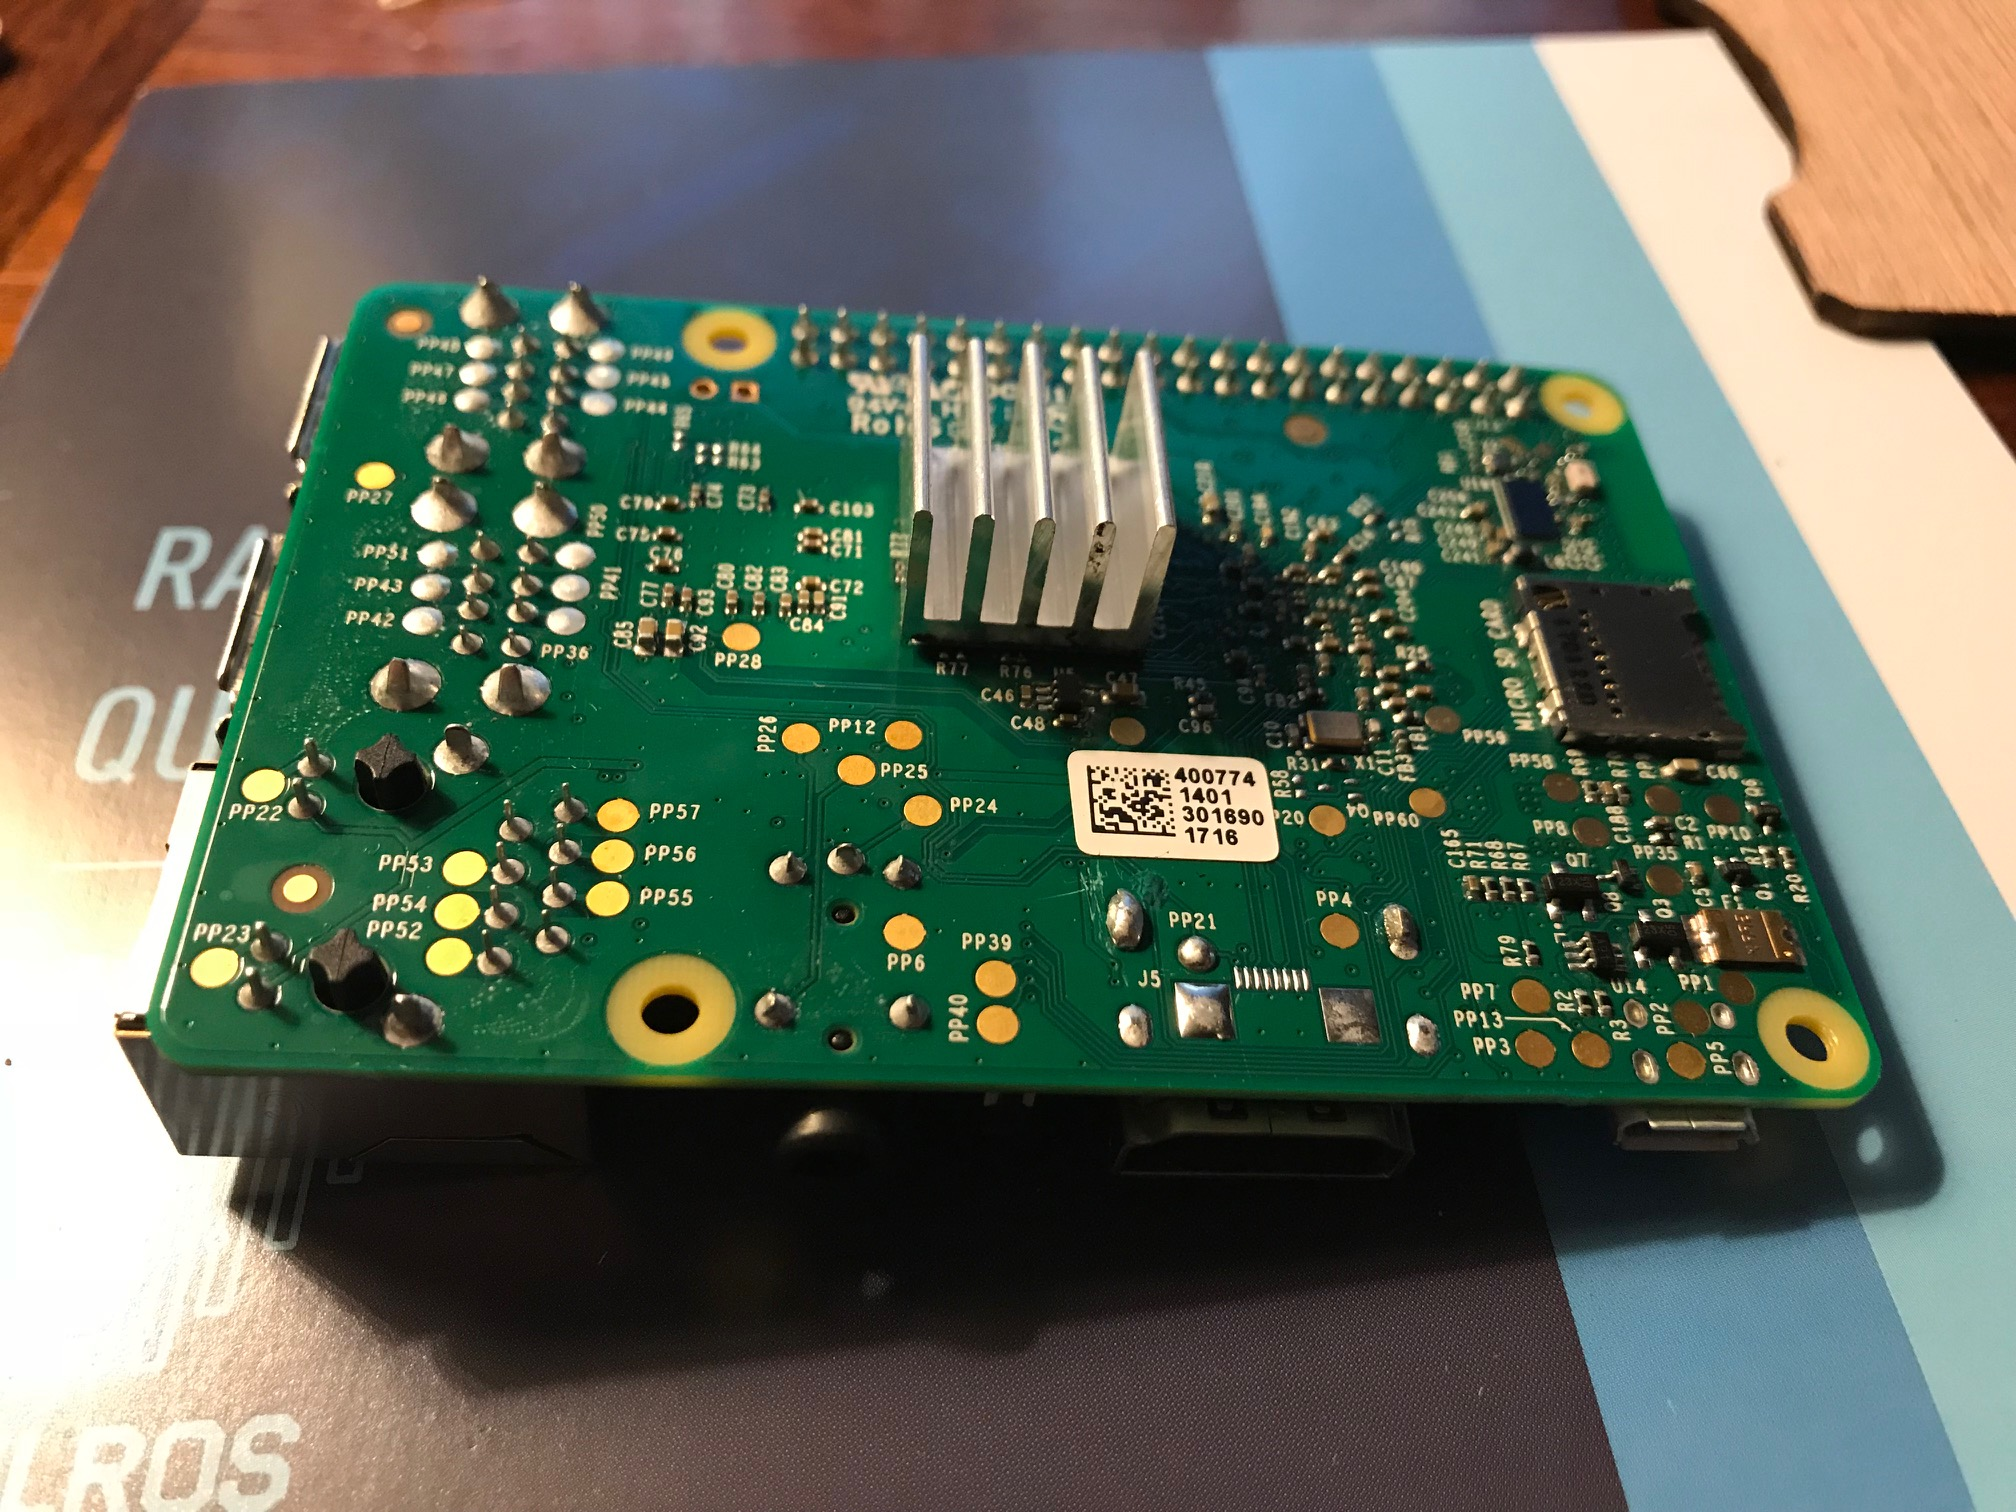
\includegraphics[width=0.6\columnwidth]{images/RASP3_1.jpg}}
    \caption{Unboxed Raspberry Pi 3 with heatsink attached prior to mounting on case bottom}\label{F:rasp}
%\end{figure}

\bigskip

%\begin{figure}[htb]
    {\centering
    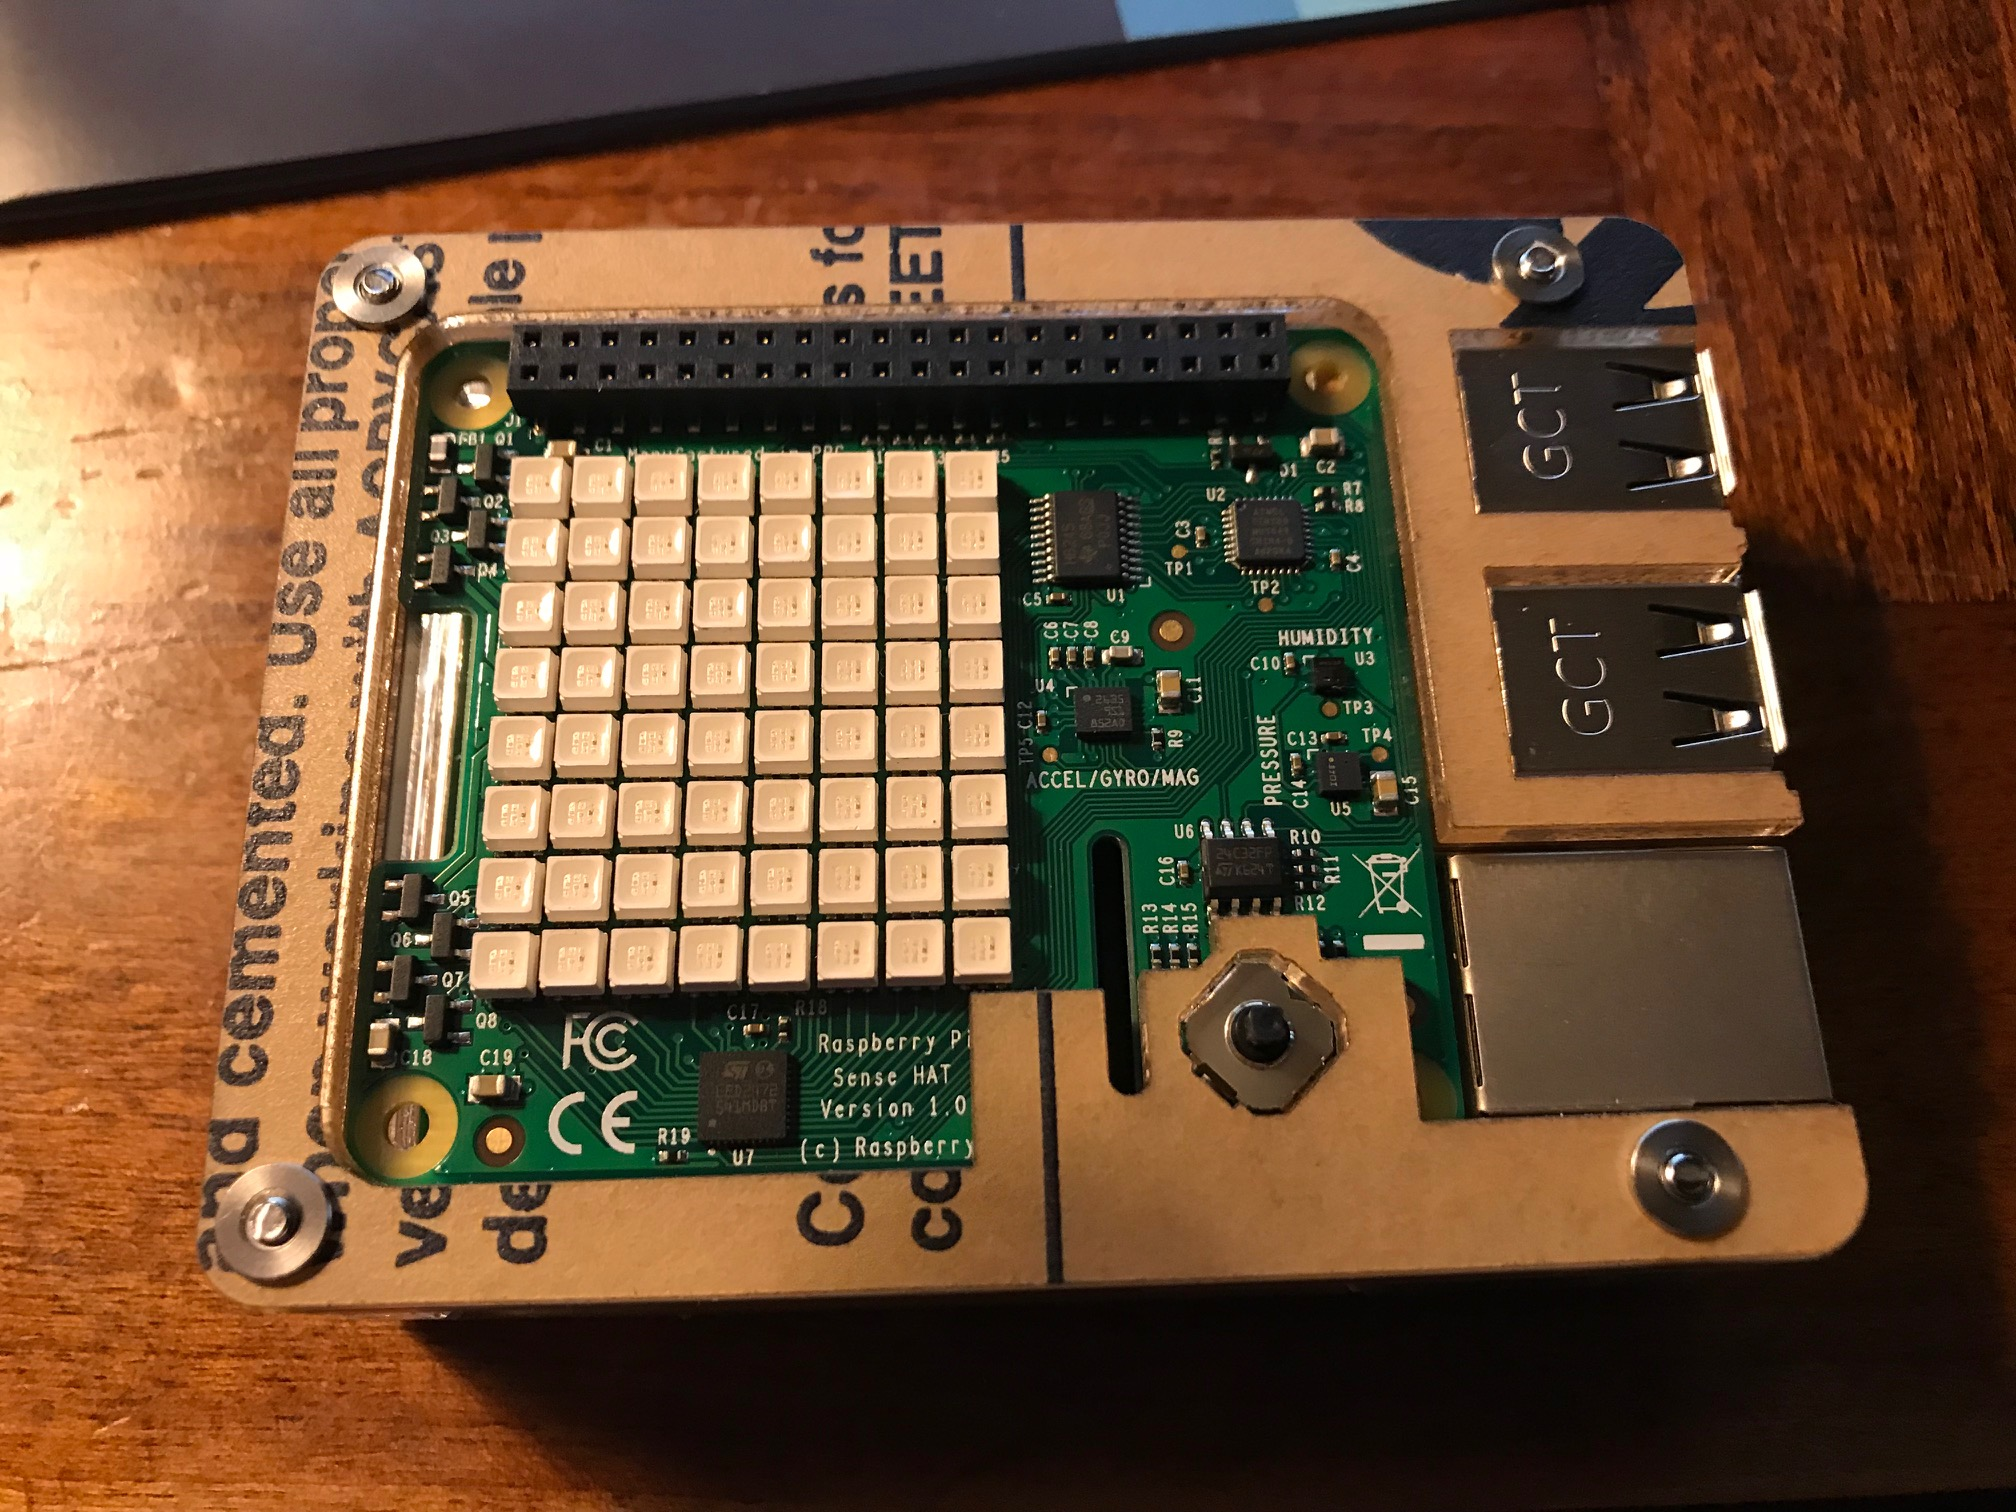
\includegraphics[width=0.6\columnwidth]{images/SENSE_Case1.jpg}}
    \caption{Sense Hat attached to the Raspberry Pi 3 with the Zebra Case assembled upward from the bottom in layers}
%\end{figure}

\bigskip

%\begin{figure}[htb]
    {\centering
    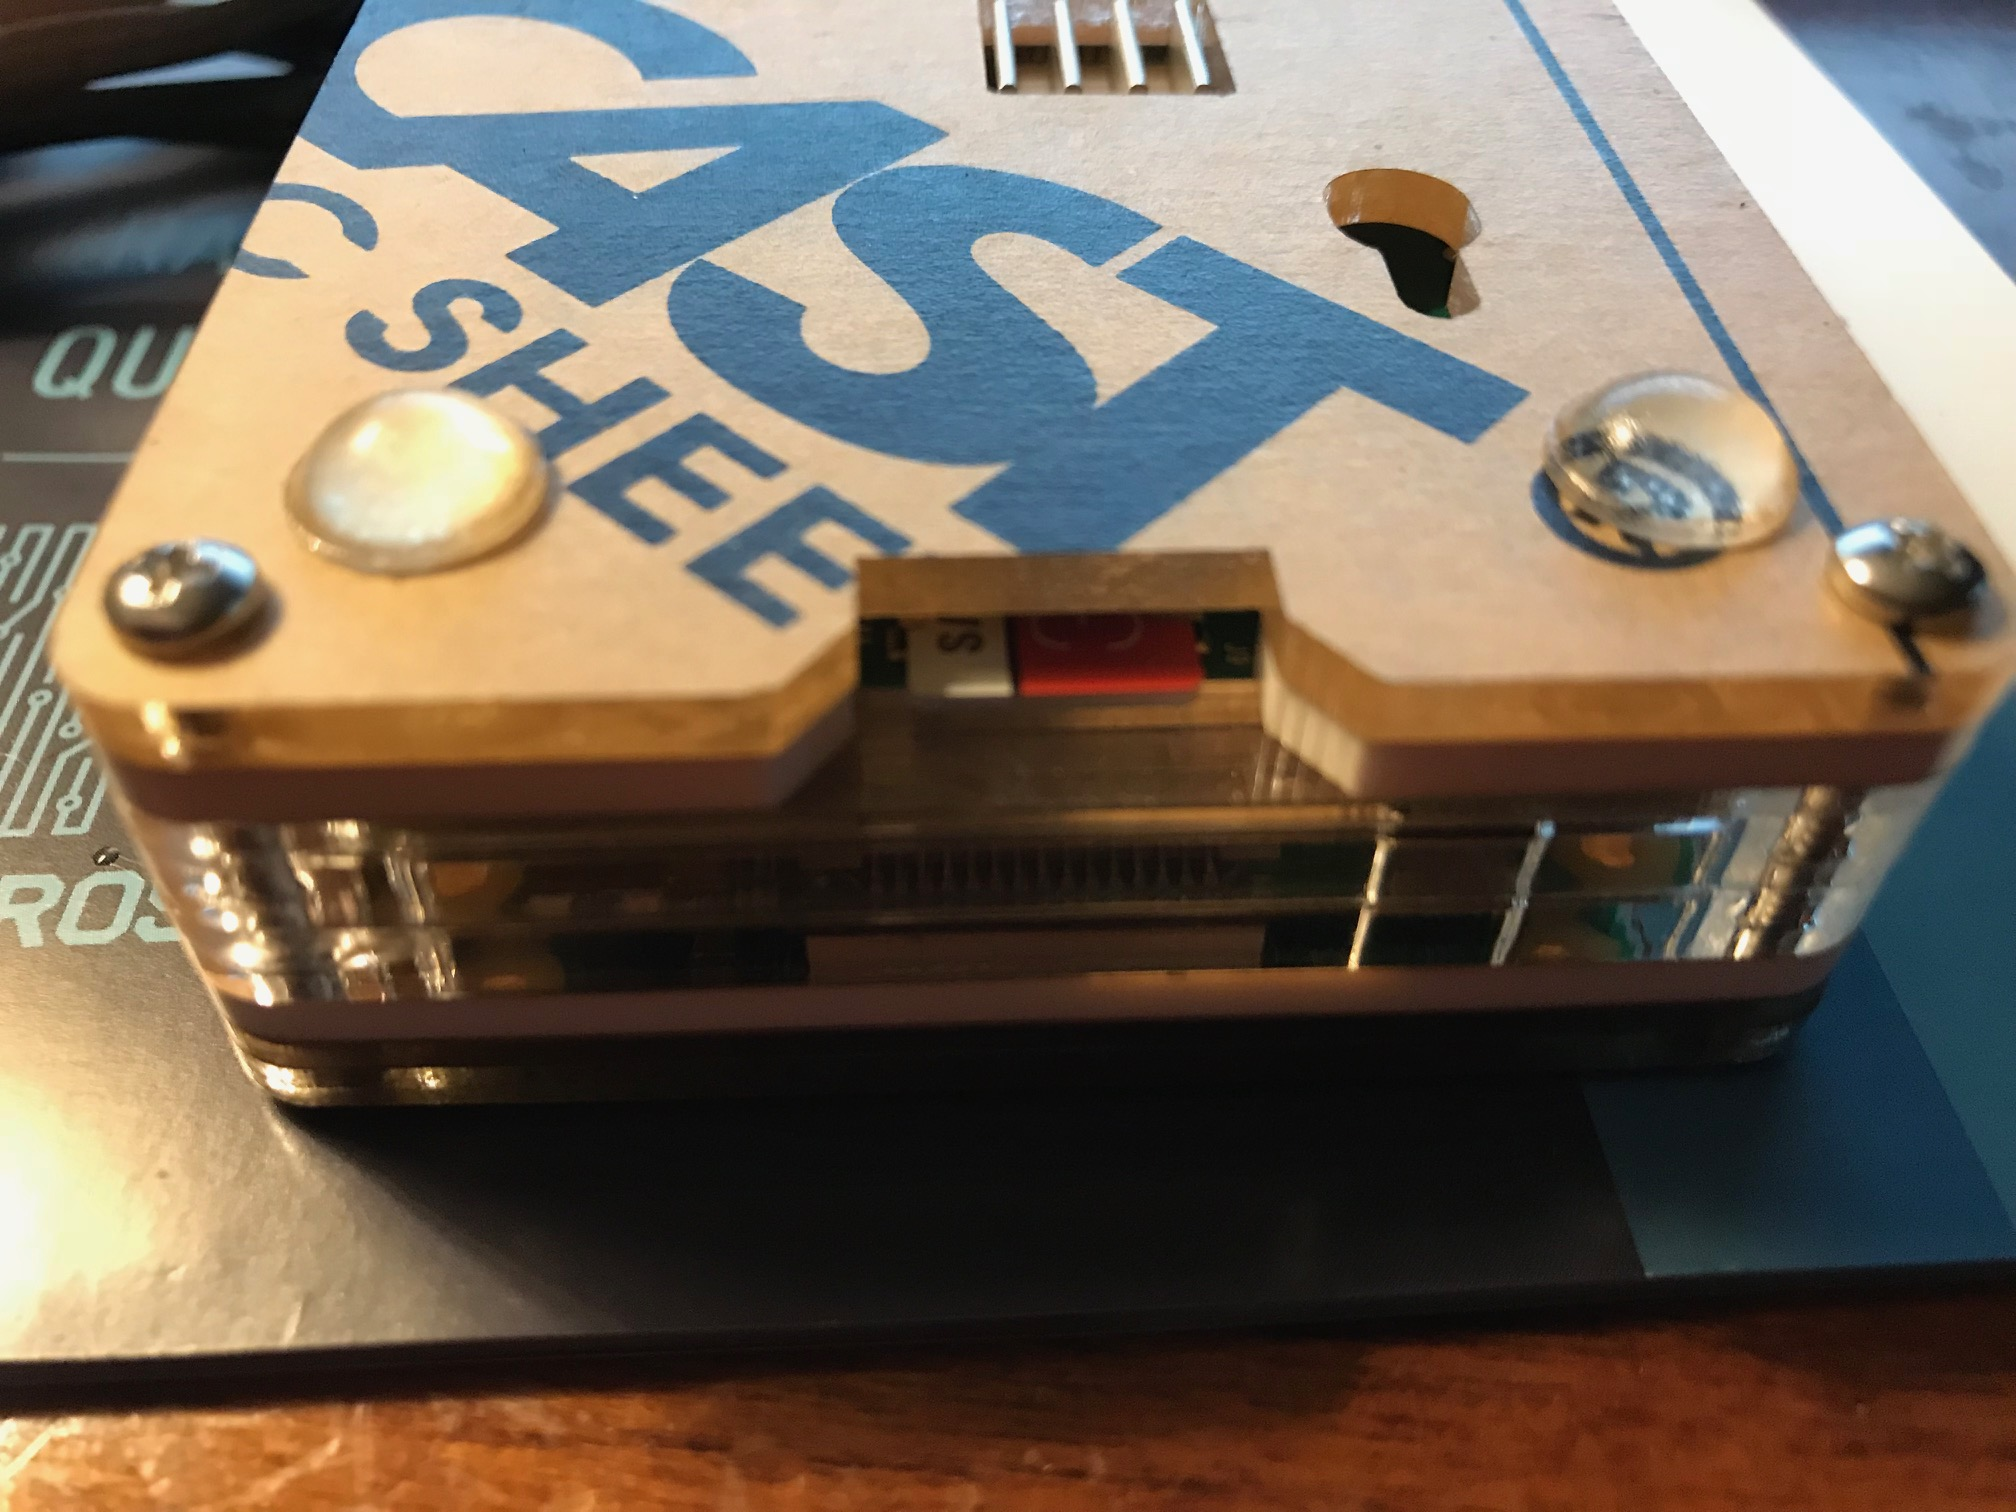
\includegraphics[width=0.6\columnwidth]{images/Bottom_Case.jpg}}
    \caption{SD Card inserted through the slot on the bottom of the PWS}
%\end{figure}

\bigskip

%\begin{figure}[htb]
    {\centering
    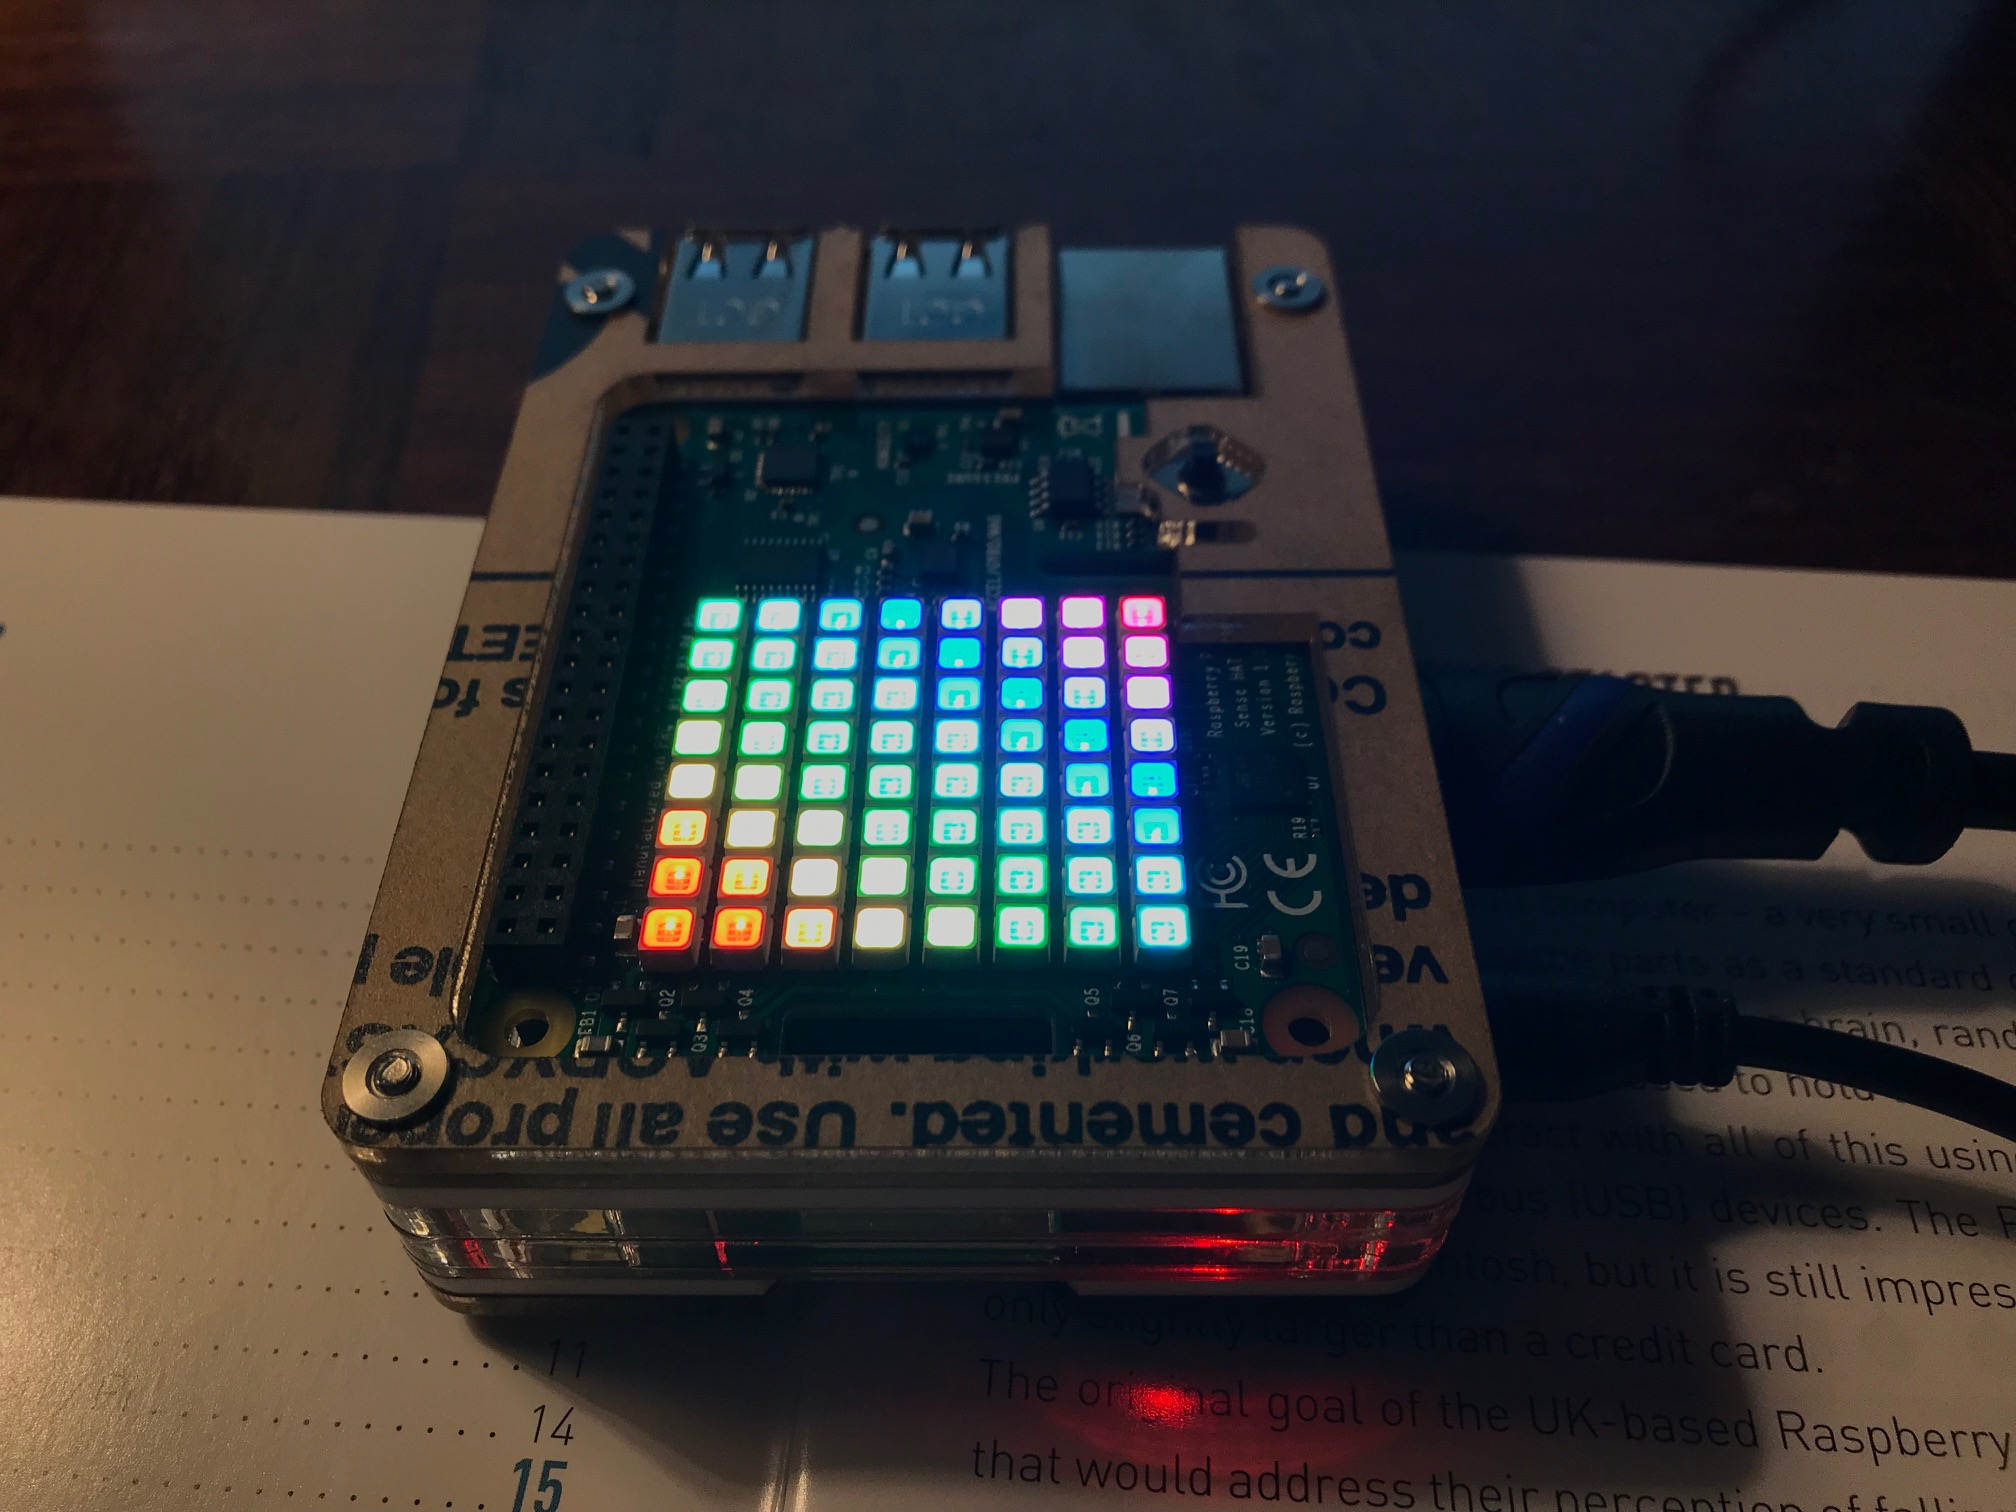
\includegraphics[width=0.6\columnwidth]{images/ON.jpg}}
    \caption{PWS powered on for the first time}
\end{figure}


\section{Initial Configuration of the Raspberry Pi 3}

After building the physical infrastructure of the PWS, it was configured with the NOOBS operating system that was pre-loaded on the mini SD card and then updates were installed. These were the steps that were followed:



\begin{figure}[htb]
    \centering
    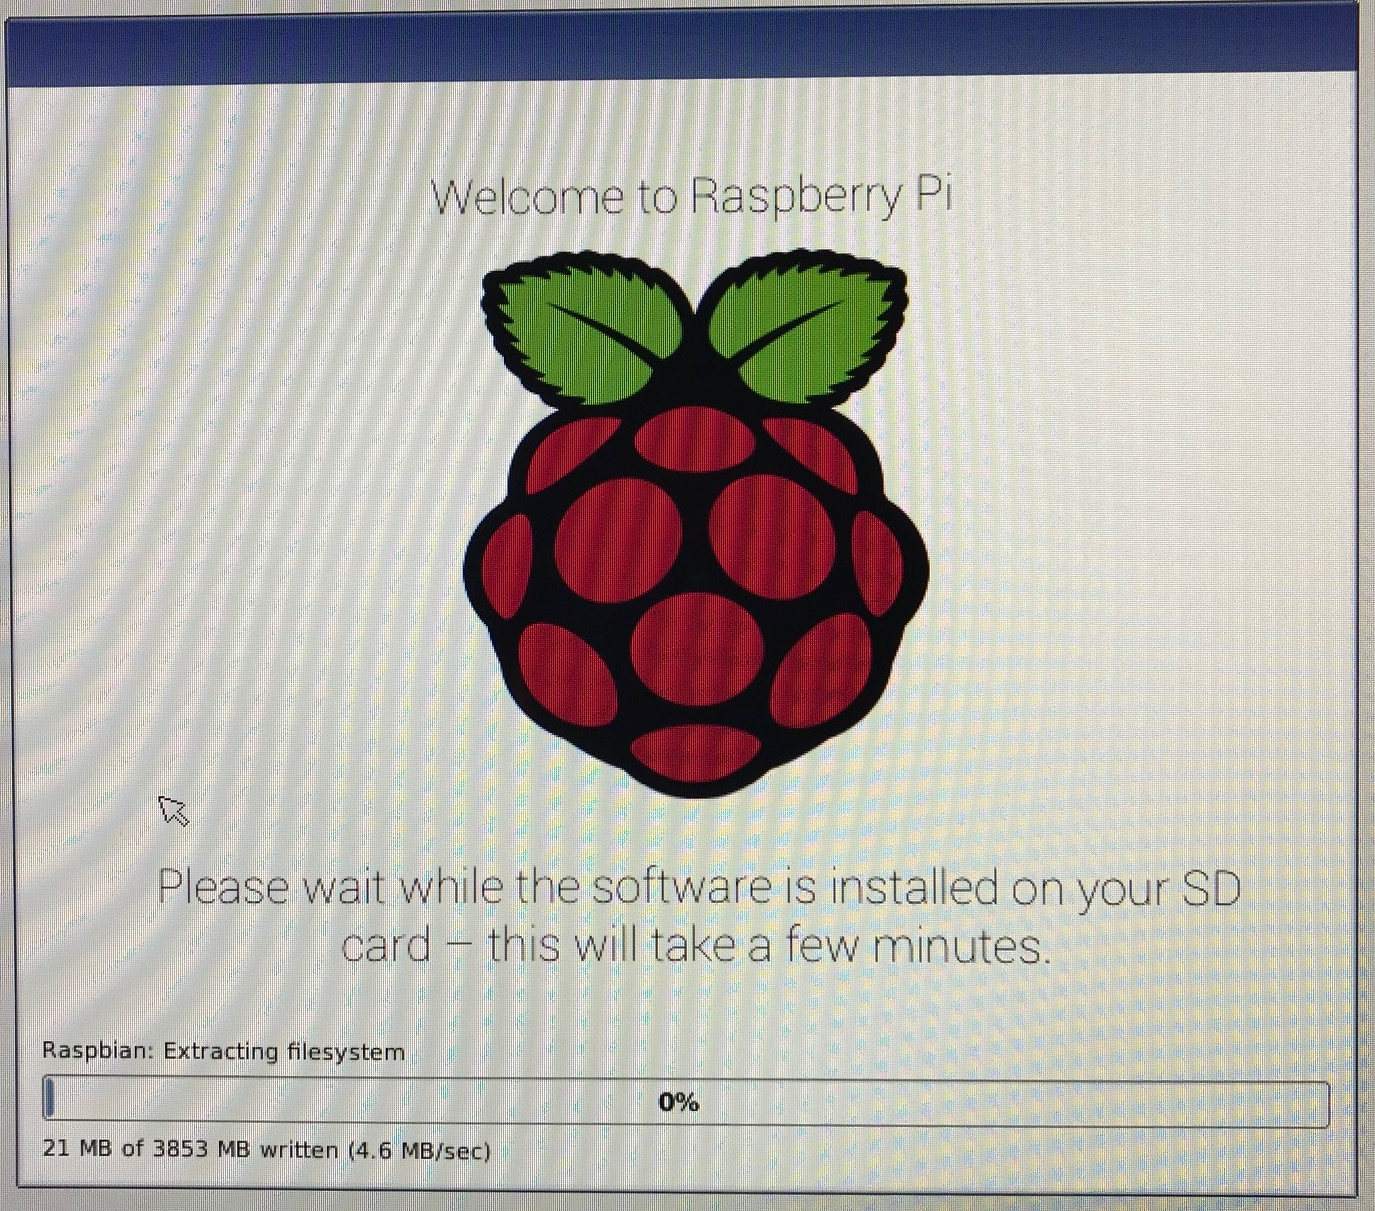
\includegraphics[width=0.5\columnwidth]{images/Raspbian_Boot.jpg}
    \caption{NOOBS OS is in the process of installing}
\end{figure}

\begin{enumerate}
\item Plugged mini USB plug into the Raspberry Pi 3.
\item Plugged peripherals (monitor, keyboard, mouse) into the Raspberry Pi 3.
\item The device booted and began automatically installing the NOOBS operating system.
\item After NOOBS completed its installation, the Raspberry Pi preferences could be configured. 
\item By selecting Preferences -> Raspberry Pi Configuration, disk space could then be expanded by clicking the "Expand Filesystem" button. This was required because the default setup ultimately leaves too little disk space for all the software required for the project. SHOW IMAGE
\item The hostname can also be renamed so that it can easily be found on your home WiFi network.
\item It's also a good idea to update the Raspberry Pi 3's software, which was done by opening a terminal window entering the following command - which updates the Raspberry Pi 3's indexes of the most up-to-date software packages:


\begin{verbatim}
sudo apt-get update
\end{verbatim}

\item After software packages were updated, entering the following command then updated the Raspbian OS to the most current configuration available:

\begin{verbatim}
sudo apt-get upgrade
\end{verbatim}

\item At this point, the device was ready to begin configuration of the PWS specific software and coding.
\end{enumerate}

\section{Configuration of the Sense Hat}

Once the Raspberry Pi 3 was correctly configured, the next major step was installing and configuring the Sense Hat. Since the Sense Hat utilizes its own Python libraries, they needed to be installed as well. These were the steps that were followed:

\begin{enumerate}
\item Enter the following command to install the Sense Hat libraries:

\begin{verbatim}
sudo apt-get install sense-hat
\end{verbatim}

\item Once the Sense Hat libraries were installed, a directory was created for the Python code. This was done using the following set of commands:

\begin{verbatim}
cd ~
mkdir pi_weather_station
cd pi_weather_station
\end{verbatim}

\end{enumerate}

\section{PWS Python Source Code}

Overall the Python source code used for this project is fairly straightforward\cite{WundergroundPython2017}. In essence, it is telling the Sense Hat to measure temperature, humidity, and pressure during specific intervals and to send them to Weather underground. 

\TODO{You need a sentence with the Figure \ref{F:upload}. Long code must be in a figure}

\begin{figure}[htb]
\begin{verbatim}
if WEATHER_UPLOAD:
  print("Uploading data to Weather Underground")
    weather_data = {
      "action": "updateraw",
      "ID": wu_station_id,
      "PASSWORD": wu_station_key,
      "dateutc": "now",
      "tempf": str(temp_f),
      "humidity": str(humidity),
      "baromin": str(pressure),
      }
      try:
        upload_url = WU_URL + "?" + urlencode(weather_data)
        response = urllib2.urlopen(upload_url)
        html = response.read()
        print("Server response:", html)
        response.close() 
    except:
      print("Exception:", sys.exc_info()[0], SLASH_N)
    else:
      print("Skipping Weather Underground upload")
\end{verbatim}
\caption{YOUR CAPTION HERE}\label{F:upload}
\end{figure}

The code also makes use of the Sense Hat's 8X8 full-color LED matrix to display with a "W" for Warmer if the moving average of the temperature has increased since the past interval or a "C" for Cooler if the moving average of the temperature has decreased since the past interval. If the moving average of the temperature remains the same since the past interval, it displays a red and blue equal sign for no change in temperature. 

\begin{verbatim}
b = [0, 0, 255]  # blue
r = [255, 0, 0]  # red
e = [0, 0, 0]  # empty
warm_up = [
    r, r, e, r, r, e, r, r,
    r, r, r, r, r, e, r, r,
    r, r, e, r, r, e, r, r,
    r, r, e, r, r, e, r, r,
    r, r, e, r, r, e, r, r,
    r, r, e, r, r, e, r, r,
    r, r, r, r, r, r, r, r,
    e, r, r, r, r, r, r, e
]
cool_down = [
    e, b, b, b, b, b, b, e,
    b, b, b, b, b, b, b, b,
    b, b, e, b, b, e, b, b,
    b, b, e, b, b, e, e, e,
    b, b, e, b, b, e, e, e,
    b, b, e, b, b, e, b, b,
    b, b, b, b, b, b, b, b,
    e, b, b, b, b, b, b, e
]
bars = [
    e, e, e, e, e, e, e, e,
    e, e, e, e, e, e, e, e,
    r, r, r, r, r, r, r, r,
    r, r, r, r, r, r, r, r,
    b, b, b, b, b, b, b, b,
    b, b, b, b, b, b, b, b,
    e, e, e, e, e, e, e, e,
    e, e, e, e, e, e, e, e
]
\end{verbatim}


There a few nuances to the code, one of which converts the standard Sense Hat measurement of temperature from Celsius to Fahrenheit and pressure from millibars to inHG. 

Celsius to Fahrenheit:

\begin{verbatim}
def c_to_f(input_temp):
    # conversion of the temp from Celsius to Fahrenheit
    return (input_temp * 1.8) + 32
\end{verbatim}


Another issue that had to be overcome was the warmth of the Raspberry Pi 3 and Sense Hat causing the temperature readings to be about 10-15 degrees warmer in Fahrenheit than the ambient temperature. Weather Underground will eventually disconnect PWSs which display erroneous and incorrect data. This was overcome by employing a "hack" available from the Pi Foundation\cite{PiFoundationHack2017}:

\begin{verbatim}
def get_temp():
    t1 = sense.get_temperature_from_humidity()
    t2 = sense.get_temperature_from_pressure()
    t = (t1 + t2) / 2
    t_cpu = get_cpu_temp()
    # Calculation for the real temperature 
    t_corr = t - ((t_cpu - t) / 1.5)
    # average over 3 readings
    t_corr = get_smooth(t_corr)
    return t_corr

def main():
    global last_temp
    last_minute = datetime.datetime.now().minute
    last_minute -= 1
    if last_minute == 0:
        last_minute = 59
\end{verbatim}


Another nuance to the data collection aspect is the moving average. Though the PWS is only sending weather data to Weather Underground every 10 minutes, it is reading the data locally on the device every 5 seconds and sending the moving average to Weather Underground. 


\begin{verbatim}
def get_smooth(x):
    if not hasattr(get_smooth, "t"):
        get_smooth.t = [x, x, x]
    get_smooth.t[2] = get_smooth.t[1]
    get_smooth.t[1] = get_smooth.t[0]
    get_smooth.t[0] = x
    # average of the last 3 smooth temps
    xs = (get_smooth.t[0] + \
          get_smooth.t[1] + \
          get_smooth.t[2]) / 3
    return xs
\end{verbatim}


For this project, the above source code was saved as 

\verb|personal_weather_station.py| 

and placed in the 

\verb|pi_weather_station| 

 directory that was created during steps we did for configuring the Sense Hat. In addition to the \verb|personal_weather_station.py| code, a configuration file is also required in order for the PWS to be able to interface with Weather Underground. The configuration file is fairly simple, comprised of just 3 lines of code:


\begin{verbatim}
class Config:
    STATION_ID = ""
    STATION_KEY = ""
\end{verbatim}


Both the Station ID and the Station Key are obtained when setting up an account on Weather Underground. More on that next.

\section{Registering the PWS on Weather Underground}

Why Weather Underground? Weather Underground started in 1995 as an internet weather service, initially with the sole purpose of displaying real-time weather data on the web. By 2012 the Weather Channel (The Weather Company) had acquired Weather Underground and by 2017 Weather Underground had over 260,000+ PWSs feeding weather data into its cloud-based weather tracking and analysis system. These observations are used in conjunction with official National Weather Service weather stations to provide very detailed and dynamically-updated features on Weather Underground and Weather Channel's forecasting service as well as Google's Map base.

Setting up a PWS on Weather Underground network wasn't particularly difficult, but some basic requirements need to be met. First, the PWS of choice must be able to interface with Weather Underground's servers. The Raspberry Pi 3 and Sense Hat are perfect for this and hence why they were used for this project. The following are the steps that were followed for setting up the device:

\begin{enumerate}
    \item From the http://www.wunderground.com web page, an account must be registered following the standard procedure for doing something like this. Given that the PWS that was registered is keyed into a particular geographic location, an address as well as elevation must be provided. 
    \item A name was also picked for the PWS, and for the purposes of this project, the name "Deer Ridge" was selected.
\end{enumerate}

After completing these steps, the Station ID and Station Access Key were provided but were not yet entered into the config.py file in the \verb|pi_weather_station| directory on the PWS. It was only after successful completion of testing and automation that this final step was taken.

\section{Initial Testing and Automation}

Prior to placing the PWS outside (where it will no longer be easy to plug in its peripherals), some initial testing was conducted before automating the startup of the \verb|personal_weather_station.py| script and submitting potentially false and inaccurate data to Weather Underground. It was also during this testing that the Sense Hat warm temperature sensor issue first presented itself and it was determined that it needed to be fixed prior to configuring the device to send data to Weather Underground. 

After plugging in the device and manually launching the main source code script, it was confirmed that the script was working as expected, including the readouts on the LED matrix display. Data began populating at 5 second intervals in the terminal window and the correct readouts were displaying on the LED matrix. However, according to the Nest in my home the ambient temperature in the house was 70 degrees Fahrenheit. Yet the PWS was registering at 81 degrees Fahrenheit and climbing. Thus, as it was explained in the above section on the project source code, a workaround had to be implemented in the code to compensate for this temperature. 

Once that issue was resolved, it was time to configure the PWS scripts to run automatically upon PWS startup. The advantages to doing this allowed the PWS to be moved (unplugged from its power source) and to maintain a constant stream of weather data to Weather Underground in the event of a power outage or WiFi reboot. 

This automated startup can be accomplished by opening a terminal window and navigating to the \verb|pi_weather_station| directory on the PWS. Once there, the project's Bash script file can be turned into an executable using the following command:


\begin{verbatim}
    chmod +x start-station.sh
\end{verbatim}


Once this command was entered, then the autostart file can be opened and the following line of code can be added:


\begin{verbatim}
@lxterminal -e /home/pi/pi_weather_station/start-station.sh
\end{verbatim}



After rebooting the PWS, the \verb|personal_weather_station.py| then started automatically. The script was then stopped and the Station ID and Station Access Key that were provided by Weather Underground during registration were entered into the config.py file in the \verb|pi_weather_station| directory on the PWS.

\section{PWS Location Selection}

Before turning on the PWS and transmitting data to Weather Underground, a suitable location needed to be selected for the PWS. The basic requirements for this were that the sensors need to be as out in the open and exposed to the outdoor elements as much as possible while also not getting wet or exposed to too much wind and dust. Weather Underground suggests placement of at least 5 feet off the ground and away from concrete, asphalt, and any other heat-producing appliances such as air conditioners or solar inverters. 

The most reasonable location available for this project was the inside of a fence post, tucked under the eves of the house. This way, the PWS was not in direct sunlight, in danger of getting wet, and also near a power supply. The PWS was mounted on the fence post about 5 feet off the ground and plugged into a power source. 

\begin{figure}[htb]
    \centering
    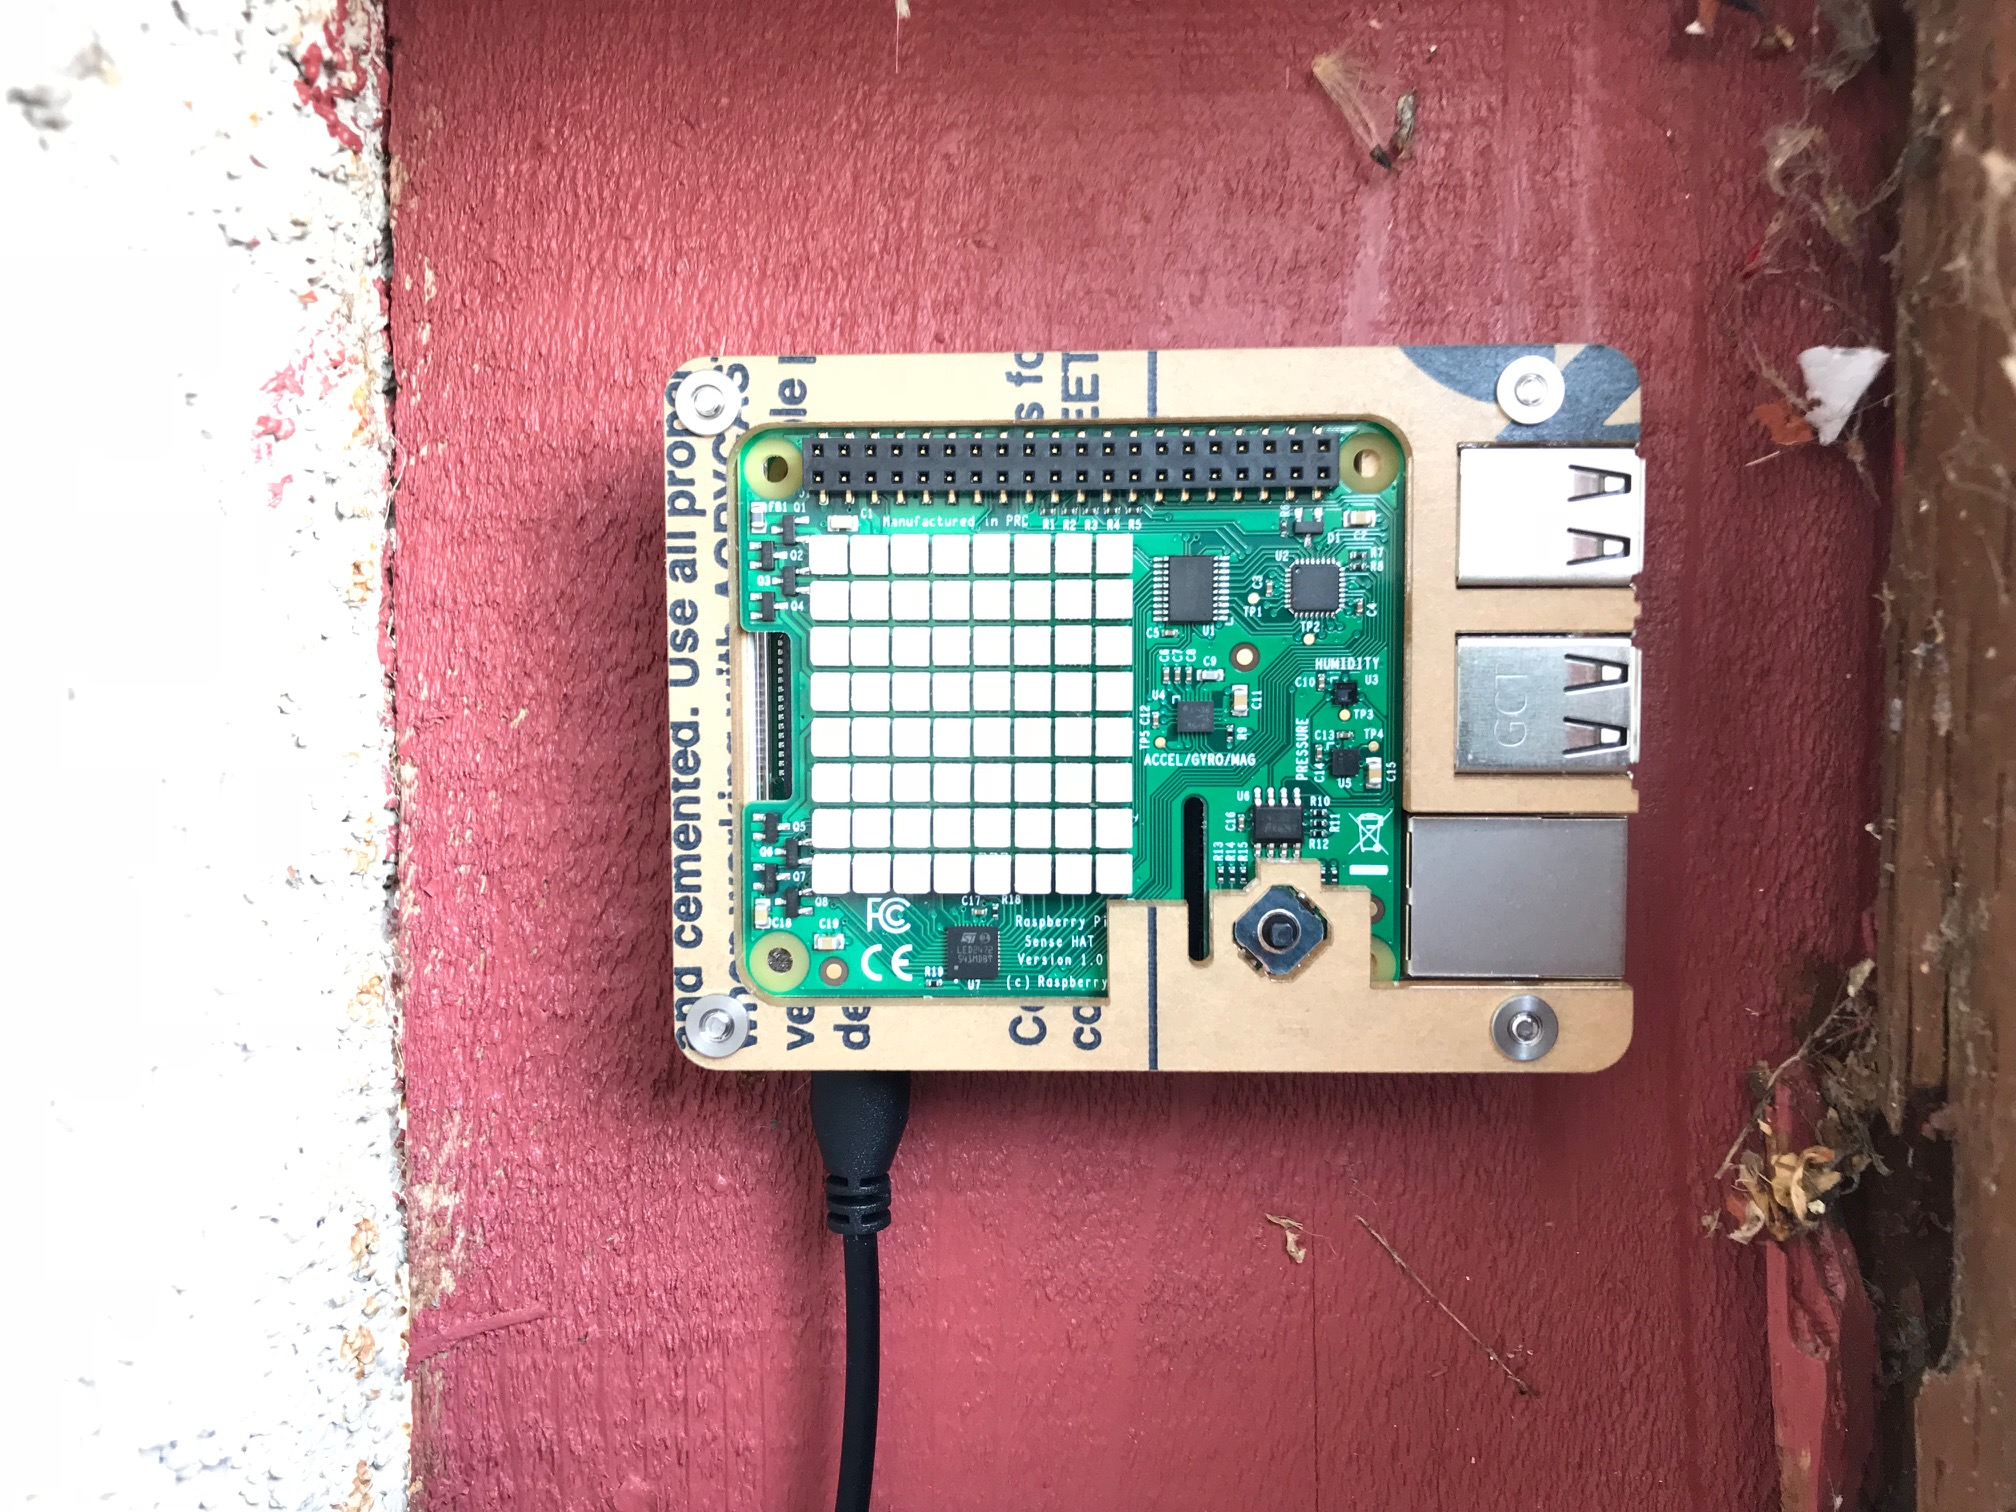
\includegraphics[width=\columnwidth]{images/Location1.jpg}
    \caption{PWS mounted in an outdoor, protected area, out of direct sunlight}
\end{figure}

The geographic location chosen for the PWS was Northern California with the time setting for this project over the course of an 8 day period during the month of November, from 11/21/2017 to 11/28/2017. This is a time in which weather conditions in this part of the country are in flux and make for some interesting readings. The PWS is also at roughly 300 feet of elevation in the foothills east and in the rain shadow of large mountain with approximately 4,000 feet of elevation. The PWS is located roughly 60 miles east of the Pacific Ocean and therefore is exposed to rapidly changing weather patterns in the fall. These patterns are born out in the data.

\section{Official Weather Data Source Selection}

Both the geography and topography of the area around the site of the PWS built for this project vary greatly within 1-5 miles let alone 10-20 miles. Roughly half of the people who live in the United States live within 17 miles of an airport, while 90 percent live within 58 miles of an airport.\cite{Pearson2017} In nearly all cases, airports are equipped with the most advanced weather station and data collection technology, so they are often most cited for their data. As an official weather source for this project, the KSCK Stockton Airport WS weather station is 31 miles away and is the closest major airport to the location of the PWS built for this project. The Stockton Airport WS weather station collects a variety of comprehensive weather data, though for this project, we are only comparing temperature, humidity, and pressure. 


\section{Addition PWS Data Selection}

In addition to the official weather source from Stockton Airport WS, 3 additional PWSs in varying proximity to the Deer Ridge PWS (but not further away than Stockton Airport WS) were selected to collect temperature, humidity, and pressure data for a date range of 11/21/2017 to 11/28/2017. The stations selected were (ordered by distance from Deer Ridge PWS):

\section{Addition PWS Data Selection} 

\subsection{Deer Ridge Country Club PWS}

Type: Netatmo Weather Station, located less than 1 mile from the Deer Ridge PWS at an elevation of 173 feet.

\begin{figure}[htb]
    \centering
    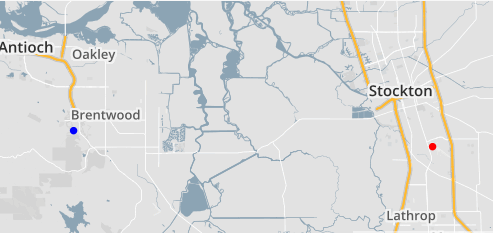
\includegraphics[width=\columnwidth]{images/DR_Stockton.PNG}
    \caption{Location of the Deer Ridge PWS (Blue Dot in relation to Stockton Airport PWS (Red Dot)}
    \label{Image 1: Deer Ridge}
\end{figure}

\begin{figure}[p]
    \centering
    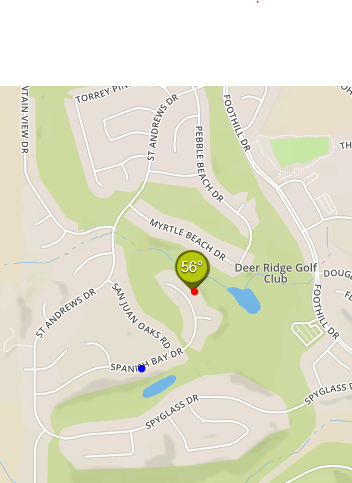
\includegraphics[width=.56\columnwidth]{images/DR_DRCC.PNG}
    \caption{Location of Deer Ridge PWS (Blue Dot) in relation to Deer Ridge Country Club PWS (Red Dot)}
%\end{figure}

\bigskip

%\begin{figure}[htb]
    \centering
    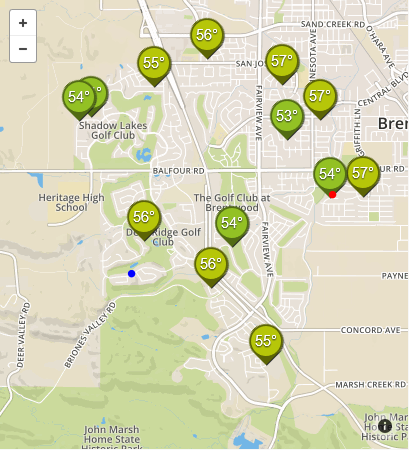
\includegraphics[width=.56\columnwidth]{images/DR_Campinello.PNG}
    \caption{Location of Deer Ridge PWS (Blue Dot) in relation to Campanello PWS (Red Dot)}
%\end{figure}

\bigskip

%\begin{figure}[htb]
    \centering
    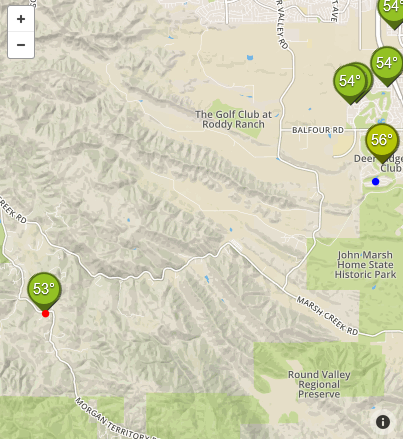
\includegraphics[width=.56\columnwidth]{images/DR_MTP.PNG}
    \caption{Location of Deer Ridge PWS (Blue Dot) in relation to Morgan Territory PWS (Red Dot)}
\end{figure}


\subsection{Campanello PWS}

Type: Netatmo Weather Station, located 2.2 miles from the Deer Ridge PWS at an elevation of 88 feet.


\subsection{Morgan Territory PWS} 

Type: AcuRite Pro Weather Center, located 4.8 miles from the Deer Ridge PWS at an elevation of 820 feet.


\section{PWS Data Analysis}

Once making these selections, collecting the data was as simple as pulling down the data from Weather Underground as each PWS and the Stockton Airport WS have their own webpages with relevant data hosted on Weather Underground.\cite{WundergroundDeerRidge2017} Data was collected in CSV format and added to the local Python Directory. Using iPython Notebook, Pandas, and Matplotlib, analysis was performed on the temperature, humidity, and pressure data collected that is useful in determining whether or not:

\begin{enumerate}
    \item Weather data coming from local PWSs is more accurate than weather data observed at the nearest major weather station, which in the case of this project, is Stockton Airport WS.
    \item Weather data coming from local PWSs can be used to interface with Nest and a Tesla Solar Array
\end{enumerate}

A total of 6 data elements were collected from 5 weather stations:

\begin{enumerate}
    \item Date
    \item Time
    \item PWS Name
    \item Temperature (Fahrenheit)
    \item Humidity (Percentage)
    \item Pressure (inHG)
\end{enumerate}

\subsection{Outliers}

The first part of the analysis that was performed as to determine if there were any outliers in the data that could, if used to feed a Nest or Tesla Solar Array, cause equipment to operate inefficiently. Obviously, given that the over-arching goal of this project is to conserve energy and allow equipment to function in the most efficient manner possible based on the most localized weather data possible, it must be determined if these sources are usable. In order to do this, Pandas was used to create a DataFrame from a CSV in iPython Notebook and Matplotlib was used to generate a bar graph. The first analysis performed was weekly record (max values) with regard to temperature, humidity, and pressure for each PWS. While the differences in pressure were negligible, there were some significant variances in both temperature and humidity, not only between the various local PWSs, but also when compared to Stockton. 

\begin{figure}[htb]
    \centering
    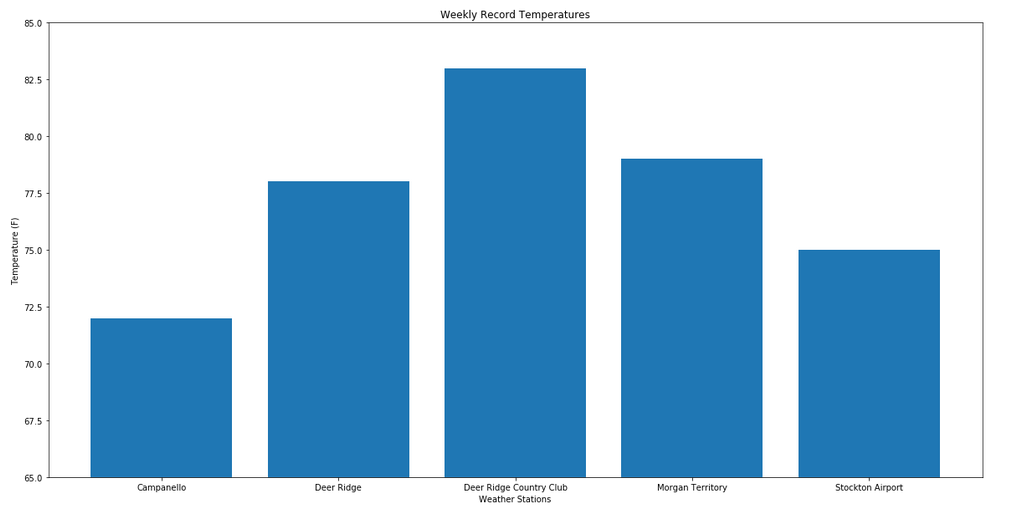
\includegraphics[width=\columnwidth]{images/WK_REC_TEMP.PNG}
    \caption{Weekly Record High Temperatures}
\end{figure}

The most significant differences were between Campanello PWS and Deer Ridge Country Club PWS, which are less than 5 miles apart and yet there was a full 12 degree difference between the two in terms of highest temperature recorded during the period in which data was collected. Another striking observation was the 5 degree difference in record high temperature between Deer Ridge PWS and Deer Ridge Country Club PWS. There is also a 5 degree difference between Campanello PWS and Deer Ridge PWS, but in the opposite direction from Deer Ridge PWS vs. Deer Ridge Country Club PWS. 

With Deer Ridge PWS falling near the average of the 5 weather stations, it would seem that the Deer Ridge Country Club PWS is either having calibration issues or is mounted in a place that is less than ideal, such as on or near a concrete surface or in direct sunlight. The Deer Ridge PWS is also closest to the Stockton Airport WS, so this is very positive news in terms of furthering the goal of obtaining the most accurate, local weather.

\begin{figure}[htb]
    \centering
    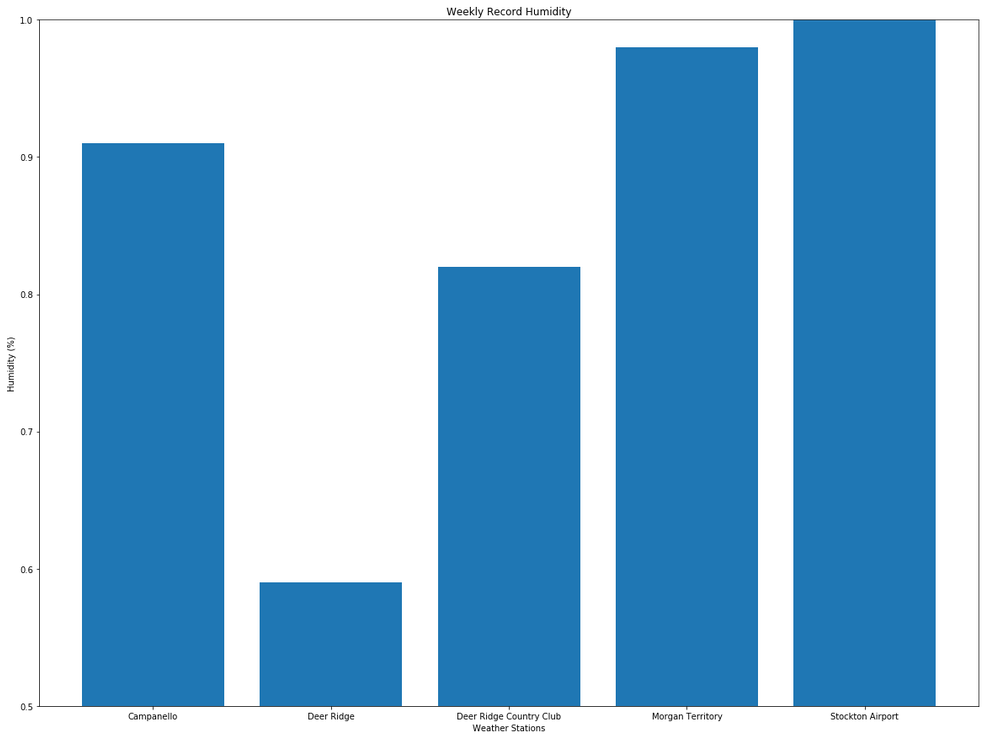
\includegraphics[width=\columnwidth]{images/WK_REC_HUM.PNG}
    \caption{Weekly Record High Humidity}
\end{figure}

With just a cursory glance at the weekly records for humidity for each of the 5 weather stations, one would have to conclude that the seems to be an issue with Stockton Airport WS. The average humidity for this part of California tends to be pretty low as the climate is generally a mix between Mediterranean/Semi-Arid. Even with the onset of the fall and winter season and the ensuing rain that comes with it, there doesn't seem to be any reasonable explanation for why Stockton Airport WS's humidity should register at greater than 70 percent more than 14 percent of the time. One explanation for this could possibly be that it has inadvertently come into contact with water, perhaps from an errant sprinkler nozzle or something similar. This might explain why the humidity hangs at 100 percent for such long periods of time and then tapers off, which is a totally unrealistic scenario. 

In fact, despite the fact that the Deer Ridge PWS seems like it is reporting low humidity, it in fact is not when compared with other PWSs that were not factored into the data, as well as from reports from the National Weather Service\cite{NWS2017}, which reported the average humidity for the period of observation to be 54 percent. This coincides with the humidity measurements that were observed on the Deer Ridge PWS, which is yet another positive aspect in proving the theory that local weather is better weather.

\subsection{PWSaaS}

Broadly speaking, PWS data would be a far better candidate for feeding IoT home devices such as Nest and a Tesla Solar Array than the currently available data from Weather Underground. As was demonstrated above, even data provided by the Stockton Airport WS contained significant outliers. Though not even other local PWSs in closer vicinity to the Deer Ridge PWS were providing accurate readings. This means that selecting the correct location for a weather station is probably even more crucial than selecting the type of equipment itself. Even with a Raspberry Pi 3 and rudimentary sensors, the data collected by it was far more close to the average than other more expensive weather stations. As was mentioned in the introduction section of this project, the cost of the Raspberry Pi 3 and its components came to less than \$100. With all of its accessories, the Netatmo PWS can cost upwards of \$ 500\cite{Netatmo2017}. The Stockton Airport WS is no doubt many thousands if not tens of thousands more than these price points, though no details are provided on Weather Underground as to type or specifications for this particular WS.

The bottom line for the Nest is that if Weather Underground can come up with an inexpensive method of certifying PWS data, it would make sense, based on the findings of this project, to release an update to their existing software that would allow Nest users to select the PWS of their choice, rather than the currently configured generic Weather Underground data. 

In terms of the Tesla Solar Array, according to Tesla's website, the only way they are currently utilizing weather data is during the design phase when they are determining feasibility for installing a solar array at client's home or business\cite{Tesla2017}:

``We will review past utility bills, sunlight patterns, and weather data for your area and create a custom system design for your home.''

What Tesla doesn't say is from where they are sourcing their data. If similar to Nest's sourcing, then Tesla's design process would also benefit from using more accurate, localized weather data. Additionally, given that Tesla solar systems are also IoT devices in that they interface both with the utility company and Tesla for the purposes of metering and monitoring, respectively, it would also be beneficial for Tesla to begin utilizing real-time weather data as well for the purposes of enhancing efficiency and energy productivity. Moreover, Nest (owned by Google) and Tesla could partner to use localized, highly accurate weather data observation and forecasting to automate two systems that manage virtually all of the energy needs of 21st century living. Personal Weather Stations as a Service (PWSaaS) could quicky become another fixture of the wired home.

\section{Conclusion}

As technology continues to progress in the 21st century, it is clear that many of the rapid advances with IoT devices once thought impossible even a decade ago are not only possible now, but are inexpensive, more accurate, and wholly underutilized. The results of this project are clear and undeniable: Individually and locally sourced weather data is far more accurate and reliable than it ever has been in the past and is clearly superior to weather data sourced from legacy weather stations at airports and meteorological centers. Given the pressing need to conserve energy and use our limited natural resources more efficiently, the need for the most accurate weather data is now far more pressing, now that IoT energy management devices such as Nest and Tesla's solar array utilize weather data for design and operation. The findings of this project are that local weather data is more accurate, but only if PWS are well-placed. This localized data will only be truly beneficial if PWSs can be certified for accuracy. If this issue of consistency can be overcome, the possibilities for integrating this data with household IoT devices are virtually limitless.

\begin{acks}

The author would like to thank Dr. Gregor von Laszewski for his support and encouragement in helping to refine the topic of this paper.

\end{acks}

\bibliographystyle{ACM-Reference-Format}
\bibliography{report} 

\end{document}
